
%(BEGIN_QUESTION)
% Copyright 2006, Tony R. Kuphaldt, released under the Creative Commons Attribution License (v 1.0)
% This means you may do almost anything with this work of mine, so long as you give me proper credit

An ingenious circuit used to generate an electrical voltage signal from a differential capacitance sensor is the {\it Twin-T diode circuit}, shown here connected to a Rosemount-style differential capacitance pressure sensor:

$$\includegraphics[width=15.5cm]{i00023x01.eps}$$

One capacitor is charged positive with respect to ground, while the other is charged negative with respect to ground, as the AC voltage source alternates positive and negative.  While one capacitor of the pressure sensor is charging, the other is discharging through $R_{load}$, producing an output voltage ($V_{out}$).

If both capacitances are equal, the output voltage will alternate equally between positive and negative values, having a DC average value of zero.  If one capacitance is larger than the other, it will store additional charge on its plates, causing it to sway the output voltage of the Twin-T circuit in the direction of its polarity.  Thus, $V_{out}$ becomes more positive as pressure increases on one side of the sensor, and more negative as pressure increases on the other side of the sensor.

\vskip 10pt

Based on this explanation of the Twin-T circuit's operation, determine which side of the pictured differential capacitance sensor is the ``High'' pressure side, and which is the ``Low'' pressure side.  Be sure to explain your reasoning!

\vfil

\underbar{file i00023}
\eject
%(END_QUESTION)





%(BEGIN_ANSWER)

This is a graded question -- no answers or hints given!

%(END_ANSWER)





%(BEGIN_NOTES)

Recall that the ``High'' pressure port of a DP instrument is that which causes the instrument's indication to become more positive when pressure is applied.  In order for this twin-T circuit to generate a more positive output voltage signal, the capacitor storing the positive charge must have greater capacitance than the capacitor storing the negative charge.  

From the orientation of the diodes, we can tell the left half of the differential capacitance cell is the capacitor storing the positive charge.  In order to make its capacitance greater, the flexible sensing diaphragm in the middle must move closer to the left stationary plate.  This means there must be greater pressure applied to the right-hand side of the cell, making the right-hand side the ``High'' pressure port side.

$$\includegraphics[width=15.5cm]{i00023x02.eps}$$



%INDEX% Measurement, pressure: differential capacitance cell

%(END_NOTES)


